\documentclass[twoside]{book}

% Packages required by doxygen
\usepackage{calc}
\usepackage{doxygen}
\usepackage{graphicx}
\usepackage[utf8]{inputenc}
\usepackage{makeidx}
\usepackage{multicol}
\usepackage{multirow}
\usepackage{textcomp}
\usepackage[table]{xcolor}

% Font selection
\usepackage[T1]{fontenc}
\usepackage{mathptmx}
\usepackage[scaled=.90]{helvet}
\usepackage{courier}
\usepackage{amssymb}
\usepackage{sectsty}
\renewcommand{\familydefault}{\sfdefault}
\allsectionsfont{%
  \fontseries{bc}\selectfont%
  \color{darkgray}%
}
\renewcommand{\DoxyLabelFont}{%
  \fontseries{bc}\selectfont%
  \color{darkgray}%
}

% Page & text layout
\usepackage{geometry}
\geometry{%
  a4paper,%
  top=2.5cm,%
  bottom=2.5cm,%
  left=2.5cm,%
  right=2.5cm%
}
\tolerance=750
\hfuzz=15pt
\hbadness=750
\setlength{\emergencystretch}{15pt}
\setlength{\parindent}{0cm}
\setlength{\parskip}{0.2cm}
\makeatletter
\renewcommand{\paragraph}{%
  \@startsection{paragraph}{4}{0ex}{-1.0ex}{1.0ex}{%
    \normalfont\normalsize\bfseries\SS@parafont%
  }%
}
\renewcommand{\subparagraph}{%
  \@startsection{subparagraph}{5}{0ex}{-1.0ex}{1.0ex}{%
    \normalfont\normalsize\bfseries\SS@subparafont%
  }%
}
\makeatother

% Headers & footers
\usepackage{fancyhdr}
\pagestyle{fancyplain}
\fancyhead[LE]{\fancyplain{}{\bfseries\thepage}}
\fancyhead[CE]{\fancyplain{}{}}
\fancyhead[RE]{\fancyplain{}{\bfseries\leftmark}}
\fancyhead[LO]{\fancyplain{}{\bfseries\rightmark}}
\fancyhead[CO]{\fancyplain{}{}}
\fancyhead[RO]{\fancyplain{}{\bfseries\thepage}}
\fancyfoot[LE]{\fancyplain{}{}}
\fancyfoot[CE]{\fancyplain{}{}}
\fancyfoot[RE]{\fancyplain{}{\bfseries\scriptsize Generated on Mon Oct 7 2013 17\-:15\-:32 for ioskj by Doxygen }}
\fancyfoot[LO]{\fancyplain{}{\bfseries\scriptsize Generated on Mon Oct 7 2013 17\-:15\-:32 for ioskj by Doxygen }}
\fancyfoot[CO]{\fancyplain{}{}}
\fancyfoot[RO]{\fancyplain{}{}}
\renewcommand{\footrulewidth}{0.4pt}
\renewcommand{\chaptermark}[1]{%
  \markboth{#1}{}%
}
\renewcommand{\sectionmark}[1]{%
  \markright{\thesection\ #1}%
}

% Indices & bibliography
\usepackage{natbib}
\usepackage[titles]{tocloft}
\setcounter{tocdepth}{3}
\setcounter{secnumdepth}{5}
\makeindex

% Hyperlinks (required, but should be loaded last)
\usepackage{ifpdf}
\ifpdf
  \usepackage[pdftex,pagebackref=true]{hyperref}
\else
  \usepackage[ps2pdf,pagebackref=true]{hyperref}
\fi
\hypersetup{%
  colorlinks=true,%
  linkcolor=blue,%
  citecolor=blue,%
  unicode%
}

% Custom commands
\newcommand{\clearemptydoublepage}{%
  \newpage{\pagestyle{empty}\cleardoublepage}%
}


%===== C O N T E N T S =====

\begin{document}

% Titlepage & ToC
\hypersetup{pageanchor=false}
\pagenumbering{roman}
\begin{titlepage}
\vspace*{7cm}
\begin{center}%
{\Large ioskj }\\
\vspace*{1cm}
{\large Generated by Doxygen 1.8.5}\\
\vspace*{0.5cm}
{\small Mon Oct 7 2013 17:15:32}\\
\end{center}
\end{titlepage}
\clearemptydoublepage
\tableofcontents
\clearemptydoublepage
\pagenumbering{arabic}
\hypersetup{pageanchor=true}

%--- Begin generated contents ---
\chapter{Main Page}
\label{index}\hypertarget{index}{}{\ttfamily ioskj} is a simulation model of the Indian Ocean skipjack tuna fishery for management strategy evaluation.

\subsection*{Status}

{\ttfamily ioskj} is still under active development. It requires several third party C++ libraries and a modern C++ compiler which supports the C++11 standard. At this stage we do not recommend trying to compile it yourself. As the model matures we intend to make it available as precompiled executables for Windows and Linux and/or a package for R.

\subsection*{Documentation}

Documentation is at \href{http://trophia.github.io/ioskj/}{\tt http\-://trophia.\-github.\-io/ioskj/}

\subsection*{Organisation}

\subsubsection*{C++ files}

The main C++ files are\-:


\begin{DoxyItemize}
\item {\ttfamily \hyperlink{dimensions_8hpp_source}{dimensions.\-hpp}} -\/ defines the dimensions used in various model arrays e.\-g. {\ttfamily Region}, {\ttfamily Age}, {\ttfamily Method}
\item {\ttfamily \hyperlink{fish_8hpp_source}{fish.\-hpp}} -\/ contains the {\ttfamily Fish} class representing the fish population dynamic
\item {\ttfamily \hyperlink{fishing_8hpp_source}{fishing.\-hpp}} -\/ contains the {\ttfamily Fishing} class representing fishing activity
\item {\ttfamily \hyperlink{data_8hpp_source}{data.\-hpp}} -\/ reads in and holds data for use in driving and conditioning the model
\item {\ttfamily \hyperlink{model_8hpp_source}{model.\-hpp}} -\/ contains the {\ttfamily Model} class which puts {\ttfamily Fish}, {\ttfamily Fishing} and the various data classes together
\item {\ttfamily main.\-cpp} -\/ the primary C++ file for compiling a {\ttfamily Model} executable
\end{DoxyItemize}

\subsubsection*{{\ttfamily data} folder}

The {\ttfamily data} folder includes R and Python scripts for processing source data. See the documentation in those files for more details. The resulting, processed data is outputted to the folder {\ttfamily data\textbackslash{}processed-\/data}.

\subsubsection*{{\ttfamily docs} folder}

The {\ttfamily docs} folder includes hand written documentation and a Doxygen project for automatically generating documentation from C++ source code/ 
\chapter{Hierarchical Index}
\section{Class Hierarchy}
This inheritance list is sorted roughly, but not completely, alphabetically\-:\begin{DoxyCompactList}
\item Data\-Group\begin{DoxyCompactList}
\item \contentsline{section}{I\-O\-S\-K\-J\-:\-:Data}{\pageref{classIOSKJ_1_1Data}}{}
\end{DoxyCompactList}
\item Dimension\begin{DoxyCompactList}
\item \contentsline{section}{I\-O\-S\-K\-J\-:\-:Data\-Year}{\pageref{classIOSKJ_1_1DataYear}}{}
\item \contentsline{section}{I\-O\-S\-K\-J\-:\-:Year}{\pageref{classIOSKJ_1_1Year}}{}
\end{DoxyCompactList}
\item \contentsline{section}{I\-O\-S\-K\-J\-:\-:Model}{\pageref{classIOSKJ_1_1Model}}{}
\item \contentsline{section}{model\-Fixture}{\pageref{structmodelFixture}}{}
\item Parameter\-Group\begin{DoxyCompactList}
\item \contentsline{section}{I\-O\-S\-K\-J\-:\-:Parameters}{\pageref{classIOSKJ_1_1Parameters}}{}
\end{DoxyCompactList}
\item \contentsline{section}{I\-O\-S\-K\-J\-:\-:Tracker}{\pageref{structIOSKJ_1_1Tracker}}{}
\end{DoxyCompactList}

\chapter{Class Index}
\section{Class List}
Here are the classes, structs, unions and interfaces with brief descriptions\-:\begin{DoxyCompactList}
\item\contentsline{section}{\hyperlink{classIOSKJ_1_1Fish}{I\-O\-S\-K\-J\-::\-Fish} }{\pageref{classIOSKJ_1_1Fish}}{}
\item\contentsline{section}{\hyperlink{classIOSKJ_1_1Fishing}{I\-O\-S\-K\-J\-::\-Fishing} }{\pageref{classIOSKJ_1_1Fishing}}{}
\item\contentsline{section}{\hyperlink{structGenerator}{Generator} }{\pageref{structGenerator}}{}
\item\contentsline{section}{\hyperlink{classIOSKJ_1_1Data_1_1MaldivePlCpue}{I\-O\-S\-K\-J\-::\-Data\-::\-Maldive\-Pl\-Cpue} }{\pageref{classIOSKJ_1_1Data_1_1MaldivePlCpue}}{}
\item\contentsline{section}{\hyperlink{classIOSKJ_1_1Model}{I\-O\-S\-K\-J\-::\-Model} }{\pageref{classIOSKJ_1_1Model}}{}
\item\contentsline{section}{\hyperlink{classIOSKJ_1_1Data_1_1NominalCatch}{I\-O\-S\-K\-J\-::\-Data\-::\-Nominal\-Catch} }{\pageref{classIOSKJ_1_1Data_1_1NominalCatch}}{}
\item\contentsline{section}{\hyperlink{classIOSKJ_1_1Data_1_1SizeFrequency}{I\-O\-S\-K\-J\-::\-Data\-::\-Size\-Frequency} }{\pageref{classIOSKJ_1_1Data_1_1SizeFrequency}}{}
\item\contentsline{section}{\hyperlink{classIOSKJ_1_1Data_1_1WestPsCpue}{I\-O\-S\-K\-J\-::\-Data\-::\-West\-Ps\-Cpue} }{\pageref{classIOSKJ_1_1Data_1_1WestPsCpue}}{}
\item\contentsline{section}{\hyperlink{classIOSKJ_1_1Data_1_1ZEstimate}{I\-O\-S\-K\-J\-::\-Data\-::\-Z\-Estimate} }{\pageref{classIOSKJ_1_1Data_1_1ZEstimate}}{}
\end{DoxyCompactList}

\chapter{Class Documentation}
\hypertarget{classIOSKJ_1_1Fish}{\section{I\-O\-S\-K\-J\-:\-:Fish Class Reference}
\label{classIOSKJ_1_1Fish}\index{I\-O\-S\-K\-J\-::\-Fish@{I\-O\-S\-K\-J\-::\-Fish}}
}
\subsection*{Public Member Functions}
\begin{DoxyCompactItemize}
\item 
void \hyperlink{classIOSKJ_1_1Fish_ad787d9334e8699d000825066fd546bc0}{defaults} (void)
\item 
void \hyperlink{classIOSKJ_1_1Fish_aff50e418c8b3917583430b9b421573df}{sample} (void)
\item 
void \hyperlink{classIOSKJ_1_1Fish_a5e536120fdadc3302e76270f6876cf14}{init} (void)
\item 
void \hyperlink{classIOSKJ_1_1Fish_a490ad0b072fac8f0392ecd2da9598c20}{step} (void)
\item 
\hypertarget{classIOSKJ_1_1Fish_a61462d0474ff5086919d6010a7cfdeba}{double {\bfseries biomass} (void) const }\label{classIOSKJ_1_1Fish_a61462d0474ff5086919d6010a7cfdeba}

\item 
\hypertarget{classIOSKJ_1_1Fish_aa5cd14669e73f889a3309bf824932a7e}{double {\bfseries equilibrium} (void)}\label{classIOSKJ_1_1Fish_aa5cd14669e73f889a3309bf824932a7e}

\item 
\hypertarget{classIOSKJ_1_1Fish_acc75a82f519733d425816e31b17c8fdf}{void {\bfseries write} (void)}\label{classIOSKJ_1_1Fish_acc75a82f519733d425816e31b17c8fdf}

\end{DoxyCompactItemize}
\subsection*{Public Attributes}
\begin{DoxyCompactItemize}
\item 
\hypertarget{classIOSKJ_1_1Fish_a1bb94657937a5693877ffcda2aa05484}{Array$<$ double, Region, Age, Size $>$ {\bfseries numbers}}\label{classIOSKJ_1_1Fish_a1bb94657937a5693877ffcda2aa05484}

\item 
\hypertarget{classIOSKJ_1_1Fish_aee795e04e3454a81acf2e883a23baae0}{double {\bfseries r0}}\label{classIOSKJ_1_1Fish_aee795e04e3454a81acf2e883a23baae0}

\item 
\hypertarget{classIOSKJ_1_1Fish_a346a8928285d63ac27b5c867055e0531}{double {\bfseries recruit\-\_\-sd}}\label{classIOSKJ_1_1Fish_a346a8928285d63ac27b5c867055e0531}

\item 
\hypertarget{classIOSKJ_1_1Fish_aa75b964e87b21f46632974f15d97a32a}{bool {\bfseries recruit\-\_\-var}}\label{classIOSKJ_1_1Fish_aa75b964e87b21f46632974f15d97a32a}

\item 
\hypertarget{classIOSKJ_1_1Fish_a0776f928970167eb0aec1a5b4836b217}{bool {\bfseries recruit\-\_\-rel}}\label{classIOSKJ_1_1Fish_a0776f928970167eb0aec1a5b4836b217}

\item 
\hypertarget{classIOSKJ_1_1Fish_a8a40e0799241539b0221dc7361452083}{Array$<$ double, Size $>$ {\bfseries initials}}\label{classIOSKJ_1_1Fish_a8a40e0799241539b0221dc7361452083}

\item 
\hypertarget{classIOSKJ_1_1Fish_ab2db2279759fd69d8be56797d04c21a7}{Array$<$ double, Size $>$ {\bfseries lengths}}\label{classIOSKJ_1_1Fish_ab2db2279759fd69d8be56797d04c21a7}

\item 
\hypertarget{classIOSKJ_1_1Fish_ad999929c1154ccc87dc11d0a3dd712a8}{const double {\bfseries lengths\-\_\-step} = 2}\label{classIOSKJ_1_1Fish_ad999929c1154ccc87dc11d0a3dd712a8}

\item 
\hypertarget{classIOSKJ_1_1Fish_a2ee101f58f915ea7f431917319047afd}{double {\bfseries weight\-\_\-a}}\label{classIOSKJ_1_1Fish_a2ee101f58f915ea7f431917319047afd}

\item 
\hypertarget{classIOSKJ_1_1Fish_ab127aba9696494f34157c47c5ef29c5b}{double {\bfseries weight\-\_\-b}}\label{classIOSKJ_1_1Fish_ab127aba9696494f34157c47c5ef29c5b}

\item 
\hypertarget{classIOSKJ_1_1Fish_a5dd5a7b9ed17075f8b6ee9b000f908e2}{Array$<$ double, Size $>$ {\bfseries weights}}\label{classIOSKJ_1_1Fish_a5dd5a7b9ed17075f8b6ee9b000f908e2}

\item 
\hypertarget{classIOSKJ_1_1Fish_a47b712624f1b0f961dc30d6ad05177cc}{double {\bfseries maturity\-\_\-50}}\label{classIOSKJ_1_1Fish_a47b712624f1b0f961dc30d6ad05177cc}

\item 
\hypertarget{classIOSKJ_1_1Fish_ae69e3959280434ed86988f7c900a5802}{double {\bfseries maturity\-\_\-95}}\label{classIOSKJ_1_1Fish_ae69e3959280434ed86988f7c900a5802}

\item 
\hypertarget{classIOSKJ_1_1Fish_a35868a87508340cd35f593c1b33fad9e}{Array$<$ double, Size $>$ {\bfseries maturities}}\label{classIOSKJ_1_1Fish_a35868a87508340cd35f593c1b33fad9e}

\item 
\hypertarget{classIOSKJ_1_1Fish_a3d476797ca07a538c0000a98280131c9}{Array$<$ double, Region, Age $>$ {\bfseries mortalities}}\label{classIOSKJ_1_1Fish_a3d476797ca07a538c0000a98280131c9}

\item 
\hypertarget{classIOSKJ_1_1Fish_a09aa6f50267957567d4adcf3fdeaca93}{Array$<$ double, Region, Age, \\*
Region\-To $>$ {\bfseries movement}}\label{classIOSKJ_1_1Fish_a09aa6f50267957567d4adcf3fdeaca93}

\end{DoxyCompactItemize}


\subsection{Member Function Documentation}
\hypertarget{classIOSKJ_1_1Fish_ad787d9334e8699d000825066fd546bc0}{\index{I\-O\-S\-K\-J\-::\-Fish@{I\-O\-S\-K\-J\-::\-Fish}!defaults@{defaults}}
\index{defaults@{defaults}!IOSKJ::Fish@{I\-O\-S\-K\-J\-::\-Fish}}
\subsubsection[{defaults}]{\setlength{\rightskip}{0pt plus 5cm}void I\-O\-S\-K\-J\-::\-Fish\-::defaults (
\begin{DoxyParamCaption}
\item[{void}]{}
\end{DoxyParamCaption}
)\hspace{0.3cm}{\ttfamily [inline]}}}\label{classIOSKJ_1_1Fish_ad787d9334e8699d000825066fd546bc0}
Set default parameter values

Mainly used in testing \hypertarget{classIOSKJ_1_1Fish_a5e536120fdadc3302e76270f6876cf14}{\index{I\-O\-S\-K\-J\-::\-Fish@{I\-O\-S\-K\-J\-::\-Fish}!init@{init}}
\index{init@{init}!IOSKJ::Fish@{I\-O\-S\-K\-J\-::\-Fish}}
\subsubsection[{init}]{\setlength{\rightskip}{0pt plus 5cm}void I\-O\-S\-K\-J\-::\-Fish\-::init (
\begin{DoxyParamCaption}
\item[{void}]{}
\end{DoxyParamCaption}
)\hspace{0.3cm}{\ttfamily [inline]}}}\label{classIOSKJ_1_1Fish_a5e536120fdadc3302e76270f6876cf14}
Initialise the fish population with based on current parameter values Maturity is a logistic function of length

The fish population is initialised to an unfished state by iterating with virgin recruitment until it reaches equibrium defined by less than 0.\-01\% change in total biomass\hypertarget{classIOSKJ_1_1Fish_aff50e418c8b3917583430b9b421573df}{\index{I\-O\-S\-K\-J\-::\-Fish@{I\-O\-S\-K\-J\-::\-Fish}!sample@{sample}}
\index{sample@{sample}!IOSKJ::Fish@{I\-O\-S\-K\-J\-::\-Fish}}
\subsubsection[{sample}]{\setlength{\rightskip}{0pt plus 5cm}void I\-O\-S\-K\-J\-::\-Fish\-::sample (
\begin{DoxyParamCaption}
\item[{void}]{}
\end{DoxyParamCaption}
)\hspace{0.3cm}{\ttfamily [inline]}}}\label{classIOSKJ_1_1Fish_aff50e418c8b3917583430b9b421573df}
Sample parameter values from prior probabiity distributions \hypertarget{classIOSKJ_1_1Fish_a490ad0b072fac8f0392ecd2da9598c20}{\index{I\-O\-S\-K\-J\-::\-Fish@{I\-O\-S\-K\-J\-::\-Fish}!step@{step}}
\index{step@{step}!IOSKJ::Fish@{I\-O\-S\-K\-J\-::\-Fish}}
\subsubsection[{step}]{\setlength{\rightskip}{0pt plus 5cm}void I\-O\-S\-K\-J\-::\-Fish\-::step (
\begin{DoxyParamCaption}
\item[{void}]{}
\end{DoxyParamCaption}
)\hspace{0.3cm}{\ttfamily [inline]}}}\label{classIOSKJ_1_1Fish_a490ad0b072fac8f0392ecd2da9598c20}
Recruits are evenly distributed over regions

The documentation for this class was generated from the following file\-:\begin{DoxyCompactItemize}
\item 
/home/nbentley/\-Trophia/\-Code/ioskj/fish.\-hpp\end{DoxyCompactItemize}

\hypertarget{classIOSKJ_1_1Fishing}{\section{I\-O\-S\-K\-J\-:\-:Fishing Class Reference}
\label{classIOSKJ_1_1Fishing}\index{I\-O\-S\-K\-J\-::\-Fishing@{I\-O\-S\-K\-J\-::\-Fishing}}
}
\subsection*{Public Member Functions}
\begin{DoxyCompactItemize}
\item 
\hypertarget{classIOSKJ_1_1Fishing_a196a8e595ab828c497576419bb0f491c}{void {\bfseries init} (void)}\label{classIOSKJ_1_1Fishing_a196a8e595ab828c497576419bb0f491c}

\item 
\hypertarget{classIOSKJ_1_1Fishing_a4fe8874e2966eb554fd37b256978deb1}{void {\bfseries step} (void)}\label{classIOSKJ_1_1Fishing_a4fe8874e2966eb554fd37b256978deb1}

\end{DoxyCompactItemize}


The documentation for this class was generated from the following file\-:\begin{DoxyCompactItemize}
\item 
fishing.\-hpp\end{DoxyCompactItemize}

\hypertarget{structGenerator}{\section{Generator Struct Reference}
\label{structGenerator}\index{Generator@{Generator}}
}


{\ttfamily \#include $<$distributions.\-hpp$>$}

Inheritance diagram for Generator\-:\begin{figure}[H]
\begin{center}
\leavevmode
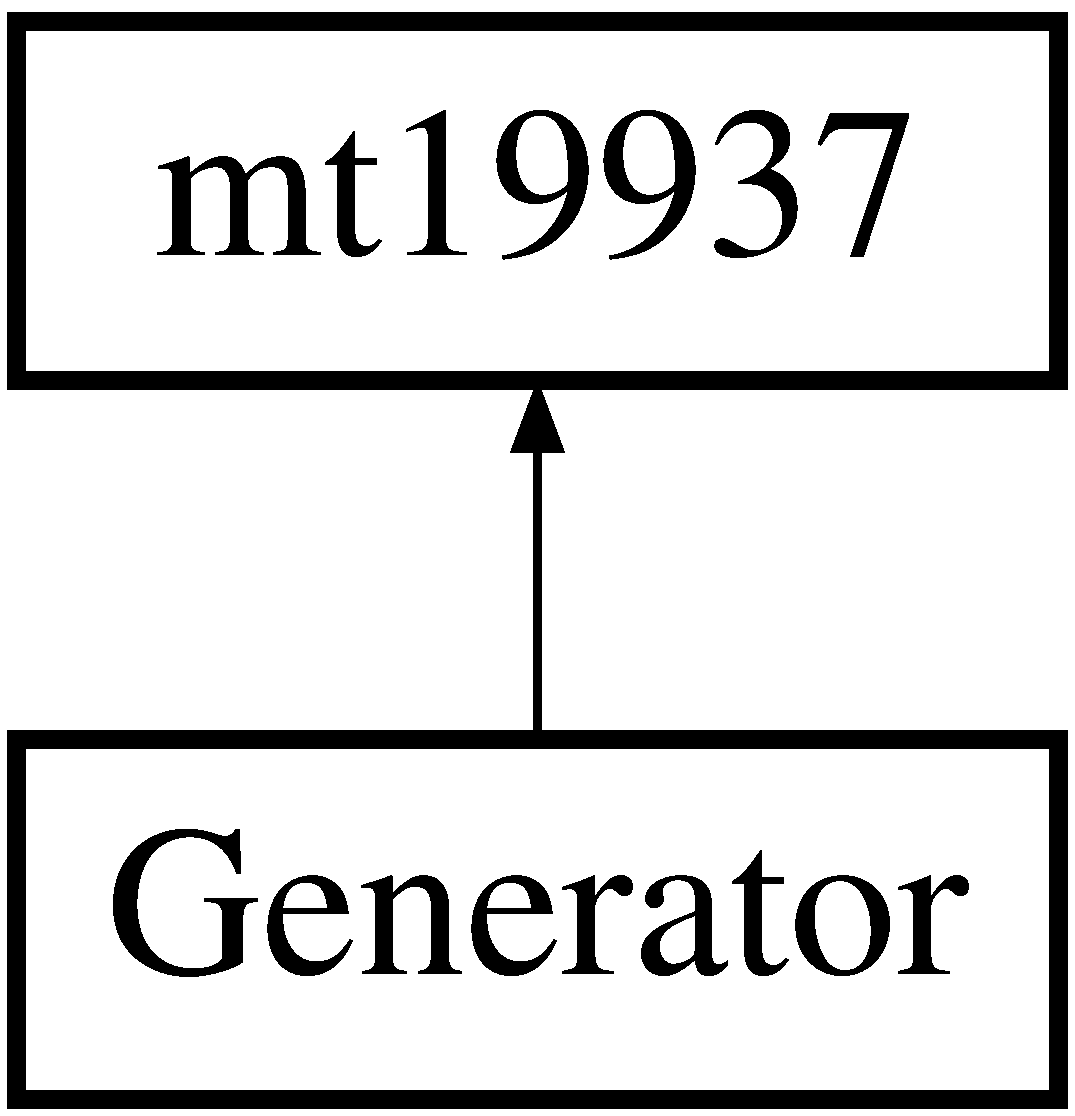
\includegraphics[height=2.000000cm]{structGenerator}
\end{center}
\end{figure}
\subsection*{Public Member Functions}
\begin{DoxyCompactItemize}
\item 
\hyperlink{structGenerator_a35e61989f22dfc623b2237ece2436dd4}{Generator} (void)
\end{DoxyCompactItemize}


\subsection{Detailed Description}
A scaffolding object that holds the random number generator used in the random() methods 

\subsection{Constructor \& Destructor Documentation}
\hypertarget{structGenerator_a35e61989f22dfc623b2237ece2436dd4}{\index{Generator@{Generator}!Generator@{Generator}}
\index{Generator@{Generator}!Generator@{Generator}}
\subsubsection[{Generator}]{\setlength{\rightskip}{0pt plus 5cm}Generator\-::\-Generator (
\begin{DoxyParamCaption}
\item[{void}]{}
\end{DoxyParamCaption}
)\hspace{0.3cm}{\ttfamily [inline]}}}\label{structGenerator_a35e61989f22dfc623b2237ece2436dd4}
Set random number generator seed using current time 

The documentation for this struct was generated from the following file\-:\begin{DoxyCompactItemize}
\item 
/home/nbentley/\-Trophia/\-Code/ioskj/distributions.\-hpp\end{DoxyCompactItemize}

\hypertarget{classIOSKJ_1_1Data_1_1MaldivePlCpue}{\section{I\-O\-S\-K\-J\-:\-:Data\-:\-:Maldive\-Pl\-Cpue Class Reference}
\label{classIOSKJ_1_1Data_1_1MaldivePlCpue}\index{I\-O\-S\-K\-J\-::\-Data\-::\-Maldive\-Pl\-Cpue@{I\-O\-S\-K\-J\-::\-Data\-::\-Maldive\-Pl\-Cpue}}
}
\subsection*{Public Member Functions}
\begin{DoxyCompactItemize}
\item 
\hypertarget{classIOSKJ_1_1Data_1_1MaldivePlCpue_a70c9b6be419fdb294f308ea5daa86aa9}{void {\bfseries read} (std\-::istream \&stream)}\label{classIOSKJ_1_1Data_1_1MaldivePlCpue_a70c9b6be419fdb294f308ea5daa86aa9}

\item 
\hypertarget{classIOSKJ_1_1Data_1_1MaldivePlCpue_a5cc13990332eef94093c2b0d4c4ac150}{void {\bfseries write} (std\-::ostream \&stream)}\label{classIOSKJ_1_1Data_1_1MaldivePlCpue_a5cc13990332eef94093c2b0d4c4ac150}

\end{DoxyCompactItemize}
\subsection*{Public Attributes}
\begin{DoxyCompactItemize}
\item 
\hypertarget{classIOSKJ_1_1Data_1_1MaldivePlCpue_a74f457be89bb489478b9361f716e52ba}{unsigned short int {\bfseries year}}\label{classIOSKJ_1_1Data_1_1MaldivePlCpue_a74f457be89bb489478b9361f716e52ba}

\item 
\hypertarget{classIOSKJ_1_1Data_1_1MaldivePlCpue_a0a933e24599d452dd116855374876bc9}{unsigned short int {\bfseries quarter}}\label{classIOSKJ_1_1Data_1_1MaldivePlCpue_a0a933e24599d452dd116855374876bc9}

\item 
\hypertarget{classIOSKJ_1_1Data_1_1MaldivePlCpue_a217bc0b50e0910ead7e0db2cbb26dc30}{float {\bfseries index}}\label{classIOSKJ_1_1Data_1_1MaldivePlCpue_a217bc0b50e0910ead7e0db2cbb26dc30}

\end{DoxyCompactItemize}


The documentation for this class was generated from the following file\-:\begin{DoxyCompactItemize}
\item 
data.\-hpp\end{DoxyCompactItemize}

\hypertarget{classIOSKJ_1_1Model}{\section{I\-O\-S\-K\-J\-:\-:Model Class Reference}
\label{classIOSKJ_1_1Model}\index{I\-O\-S\-K\-J\-::\-Model@{I\-O\-S\-K\-J\-::\-Model}}
}
\subsection*{Public Member Functions}
\begin{DoxyCompactItemize}
\item 
\hypertarget{classIOSKJ_1_1Model_ae261a53c42f71d17182c1b129698126d}{void {\bfseries track\-\_\-begin} (void)}\label{classIOSKJ_1_1Model_ae261a53c42f71d17182c1b129698126d}

\item 
\hypertarget{classIOSKJ_1_1Model_af18a3687dd2685745174b91e0aae56ce}{void {\bfseries track} (void)}\label{classIOSKJ_1_1Model_af18a3687dd2685745174b91e0aae56ce}

\item 
\hypertarget{classIOSKJ_1_1Model_a03e6aeb637c83c34774ac66c18bac74d}{void {\bfseries track\-\_\-end} (void)}\label{classIOSKJ_1_1Model_a03e6aeb637c83c34774ac66c18bac74d}

\item 
\hypertarget{classIOSKJ_1_1Model_a6f42bfc7352faa7bba7e00d04fc166b0}{void {\bfseries startup} (void)}\label{classIOSKJ_1_1Model_a6f42bfc7352faa7bba7e00d04fc166b0}

\item 
\hypertarget{classIOSKJ_1_1Model_abf9ebdb10aee501808836438cb542fab}{void {\bfseries simulate} (void)}\label{classIOSKJ_1_1Model_abf9ebdb10aee501808836438cb542fab}

\item 
\hypertarget{classIOSKJ_1_1Model_a343216d7c9019f15f01f205423001005}{void {\bfseries shutdown} (void)}\label{classIOSKJ_1_1Model_a343216d7c9019f15f01f205423001005}

\end{DoxyCompactItemize}
\subsection*{Public Attributes}
\begin{DoxyCompactItemize}
\item 
\hypertarget{classIOSKJ_1_1Model_aa8bf5f43996857e428bb0745943363a4}{\hyperlink{classIOSKJ_1_1Fish}{Fish} {\bfseries fish}}\label{classIOSKJ_1_1Model_aa8bf5f43996857e428bb0745943363a4}

\item 
\hypertarget{classIOSKJ_1_1Model_a416c537ca8c64648516e928fcea72ef2}{\hyperlink{classIOSKJ_1_1Fishing}{Fishing} {\bfseries fishing}}\label{classIOSKJ_1_1Model_a416c537ca8c64648516e928fcea72ef2}

\end{DoxyCompactItemize}


The documentation for this class was generated from the following file\-:\begin{DoxyCompactItemize}
\item 
/home/nbentley/\-Trophia/\-Code/ioskj/model.\-hpp\end{DoxyCompactItemize}

\hypertarget{classIOSKJ_1_1Data_1_1NominalCatch}{\section{I\-O\-S\-K\-J\-:\-:Data\-:\-:Nominal\-Catch Class Reference}
\label{classIOSKJ_1_1Data_1_1NominalCatch}\index{I\-O\-S\-K\-J\-::\-Data\-::\-Nominal\-Catch@{I\-O\-S\-K\-J\-::\-Data\-::\-Nominal\-Catch}}
}
\subsection*{Public Member Functions}
\begin{DoxyCompactItemize}
\item 
\hypertarget{classIOSKJ_1_1Data_1_1NominalCatch_a951b91a43b44fe8e0ade88245627a2ad}{void {\bfseries read} (std\-::istream \&stream)}\label{classIOSKJ_1_1Data_1_1NominalCatch_a951b91a43b44fe8e0ade88245627a2ad}

\item 
\hypertarget{classIOSKJ_1_1Data_1_1NominalCatch_ae32b6f662319fa27352d89e7f5918e5a}{void {\bfseries write} (std\-::ostream \&stream)}\label{classIOSKJ_1_1Data_1_1NominalCatch_ae32b6f662319fa27352d89e7f5918e5a}

\end{DoxyCompactItemize}
\subsection*{Public Attributes}
\begin{DoxyCompactItemize}
\item 
\hypertarget{classIOSKJ_1_1Data_1_1NominalCatch_a44e0f37b2fca0167eb89c4eea98785f3}{char {\bfseries area}}\label{classIOSKJ_1_1Data_1_1NominalCatch_a44e0f37b2fca0167eb89c4eea98785f3}

\item 
\hypertarget{classIOSKJ_1_1Data_1_1NominalCatch_a7c81dbf0ee1c934b6dad81477365a04e}{std\-::string {\bfseries method}}\label{classIOSKJ_1_1Data_1_1NominalCatch_a7c81dbf0ee1c934b6dad81477365a04e}

\item 
\hypertarget{classIOSKJ_1_1Data_1_1NominalCatch_a2a39b5de33deffc3bdfd20acf03be16b}{unsigned short int {\bfseries year}}\label{classIOSKJ_1_1Data_1_1NominalCatch_a2a39b5de33deffc3bdfd20acf03be16b}

\item 
\hypertarget{classIOSKJ_1_1Data_1_1NominalCatch_a480209d8d8f192a933a38aa872733131}{unsigned short int {\bfseries quarter}}\label{classIOSKJ_1_1Data_1_1NominalCatch_a480209d8d8f192a933a38aa872733131}

\item 
\hypertarget{classIOSKJ_1_1Data_1_1NominalCatch_afdcdb166bea101d81920b8508d785ebe}{float {\bfseries catches}}\label{classIOSKJ_1_1Data_1_1NominalCatch_afdcdb166bea101d81920b8508d785ebe}

\end{DoxyCompactItemize}


The documentation for this class was generated from the following file\-:\begin{DoxyCompactItemize}
\item 
data.\-hpp\end{DoxyCompactItemize}

\hypertarget{classIOSKJ_1_1Data_1_1SizeFrequency}{\section{I\-O\-S\-K\-J\-:\-:Data\-:\-:Size\-Frequency Class Reference}
\label{classIOSKJ_1_1Data_1_1SizeFrequency}\index{I\-O\-S\-K\-J\-::\-Data\-::\-Size\-Frequency@{I\-O\-S\-K\-J\-::\-Data\-::\-Size\-Frequency}}
}
\subsection*{Public Member Functions}
\begin{DoxyCompactItemize}
\item 
\hypertarget{classIOSKJ_1_1Data_1_1SizeFrequency_a47ab1ffa698fd8b3158eec2451a07b99}{void {\bfseries read} (std\-::istream \&stream)}\label{classIOSKJ_1_1Data_1_1SizeFrequency_a47ab1ffa698fd8b3158eec2451a07b99}

\item 
\hypertarget{classIOSKJ_1_1Data_1_1SizeFrequency_ae75970f485f011f5191566ca0987c572}{void {\bfseries write} (std\-::ostream \&stream)}\label{classIOSKJ_1_1Data_1_1SizeFrequency_ae75970f485f011f5191566ca0987c572}

\end{DoxyCompactItemize}
\subsection*{Public Attributes}
\begin{DoxyCompactItemize}
\item 
\hypertarget{classIOSKJ_1_1Data_1_1SizeFrequency_a08b0a6bd3c85e65f42521048e6e3bab3}{char {\bfseries area}}\label{classIOSKJ_1_1Data_1_1SizeFrequency_a08b0a6bd3c85e65f42521048e6e3bab3}

\item 
\hypertarget{classIOSKJ_1_1Data_1_1SizeFrequency_a49c0a08a3422004645d2226265c237c7}{std\-::string {\bfseries method}}\label{classIOSKJ_1_1Data_1_1SizeFrequency_a49c0a08a3422004645d2226265c237c7}

\item 
\hypertarget{classIOSKJ_1_1Data_1_1SizeFrequency_a19ef92240e288f489c5d90b1c4df0000}{unsigned short int {\bfseries year}}\label{classIOSKJ_1_1Data_1_1SizeFrequency_a19ef92240e288f489c5d90b1c4df0000}

\item 
\hypertarget{classIOSKJ_1_1Data_1_1SizeFrequency_aee8e747384c06491bebb7cc539bbb15a}{unsigned short int {\bfseries quarter}}\label{classIOSKJ_1_1Data_1_1SizeFrequency_aee8e747384c06491bebb7cc539bbb15a}

\item 
\hypertarget{classIOSKJ_1_1Data_1_1SizeFrequency_ab9833e7a7783b8b73489ac83ad0d4bd8}{std\-::array$<$ float, 61 $>$ {\bfseries props}}\label{classIOSKJ_1_1Data_1_1SizeFrequency_ab9833e7a7783b8b73489ac83ad0d4bd8}

\item 
\hypertarget{classIOSKJ_1_1Data_1_1SizeFrequency_ad494b63b6b89bdedae41e62ce4dbc1d7}{unsigned int {\bfseries num}}\label{classIOSKJ_1_1Data_1_1SizeFrequency_ad494b63b6b89bdedae41e62ce4dbc1d7}

\end{DoxyCompactItemize}


The documentation for this class was generated from the following file\-:\begin{DoxyCompactItemize}
\item 
data.\-hpp\end{DoxyCompactItemize}

\hypertarget{classIOSKJ_1_1Data_1_1WestPsCpue}{\section{I\-O\-S\-K\-J\-:\-:Data\-:\-:West\-Ps\-Cpue Class Reference}
\label{classIOSKJ_1_1Data_1_1WestPsCpue}\index{I\-O\-S\-K\-J\-::\-Data\-::\-West\-Ps\-Cpue@{I\-O\-S\-K\-J\-::\-Data\-::\-West\-Ps\-Cpue}}
}
\subsection*{Public Member Functions}
\begin{DoxyCompactItemize}
\item 
\hypertarget{classIOSKJ_1_1Data_1_1WestPsCpue_a4a66b4d327983bbcc8262cae217c7ede}{void {\bfseries read} (std\-::istream \&stream)}\label{classIOSKJ_1_1Data_1_1WestPsCpue_a4a66b4d327983bbcc8262cae217c7ede}

\item 
\hypertarget{classIOSKJ_1_1Data_1_1WestPsCpue_a21ae334f9ae536b2624e403c3b77216f}{void {\bfseries write} (std\-::ostream \&stream)}\label{classIOSKJ_1_1Data_1_1WestPsCpue_a21ae334f9ae536b2624e403c3b77216f}

\end{DoxyCompactItemize}
\subsection*{Public Attributes}
\begin{DoxyCompactItemize}
\item 
\hypertarget{classIOSKJ_1_1Data_1_1WestPsCpue_a76ed2a7cfc9dc71cd96e979a9310a4c7}{unsigned short int {\bfseries year}}\label{classIOSKJ_1_1Data_1_1WestPsCpue_a76ed2a7cfc9dc71cd96e979a9310a4c7}

\item 
\hypertarget{classIOSKJ_1_1Data_1_1WestPsCpue_a93d81fdc1e2168e56d3c7fc1173c493a}{float {\bfseries index}}\label{classIOSKJ_1_1Data_1_1WestPsCpue_a93d81fdc1e2168e56d3c7fc1173c493a}

\end{DoxyCompactItemize}


The documentation for this class was generated from the following file\-:\begin{DoxyCompactItemize}
\item 
/home/nbentley/\-Trophia/\-Code/ioskj/data.\-hpp\end{DoxyCompactItemize}

\hypertarget{classIOSKJ_1_1Data_1_1ZEstimate}{\section{I\-O\-S\-K\-J\-:\-:Data\-:\-:Z\-Estimate Class Reference}
\label{classIOSKJ_1_1Data_1_1ZEstimate}\index{I\-O\-S\-K\-J\-::\-Data\-::\-Z\-Estimate@{I\-O\-S\-K\-J\-::\-Data\-::\-Z\-Estimate}}
}
\subsection*{Public Member Functions}
\begin{DoxyCompactItemize}
\item 
\hypertarget{classIOSKJ_1_1Data_1_1ZEstimate_afd875241b51d49785e50acc239d7806e}{void {\bfseries read} (std\-::istream \&stream)}\label{classIOSKJ_1_1Data_1_1ZEstimate_afd875241b51d49785e50acc239d7806e}

\item 
\hypertarget{classIOSKJ_1_1Data_1_1ZEstimate_a952dba16d22242db687179289e576b08}{void {\bfseries write} (std\-::ostream \&stream)}\label{classIOSKJ_1_1Data_1_1ZEstimate_a952dba16d22242db687179289e576b08}

\end{DoxyCompactItemize}
\subsection*{Public Attributes}
\begin{DoxyCompactItemize}
\item 
\hypertarget{classIOSKJ_1_1Data_1_1ZEstimate_a2511cde8860fc325a4be66a05d806b94}{unsigned short int {\bfseries year}}\label{classIOSKJ_1_1Data_1_1ZEstimate_a2511cde8860fc325a4be66a05d806b94}

\item 
\hypertarget{classIOSKJ_1_1Data_1_1ZEstimate_abc1f796aef34133f4dad711ace3dd529}{unsigned short int {\bfseries quarter}}\label{classIOSKJ_1_1Data_1_1ZEstimate_abc1f796aef34133f4dad711ace3dd529}

\item 
\hypertarget{classIOSKJ_1_1Data_1_1ZEstimate_ab3cf8c05dd916758fcc22c8676473182}{float {\bfseries mu45}}\label{classIOSKJ_1_1Data_1_1ZEstimate_ab3cf8c05dd916758fcc22c8676473182}

\item 
\hypertarget{classIOSKJ_1_1Data_1_1ZEstimate_a49b0106bd644e434504ce8c677bf5d5b}{float {\bfseries mu50}}\label{classIOSKJ_1_1Data_1_1ZEstimate_a49b0106bd644e434504ce8c677bf5d5b}

\item 
\hypertarget{classIOSKJ_1_1Data_1_1ZEstimate_a7728fcde3967717cb8342ca0b0550f5d}{float {\bfseries mu55}}\label{classIOSKJ_1_1Data_1_1ZEstimate_a7728fcde3967717cb8342ca0b0550f5d}

\item 
\hypertarget{classIOSKJ_1_1Data_1_1ZEstimate_af2cdea31b63889b691238a92bca3ce10}{float {\bfseries mu60}}\label{classIOSKJ_1_1Data_1_1ZEstimate_af2cdea31b63889b691238a92bca3ce10}

\item 
\hypertarget{classIOSKJ_1_1Data_1_1ZEstimate_ac6bf29ae6cc8e5b69d21c774b5143937}{float {\bfseries sd45}}\label{classIOSKJ_1_1Data_1_1ZEstimate_ac6bf29ae6cc8e5b69d21c774b5143937}

\item 
\hypertarget{classIOSKJ_1_1Data_1_1ZEstimate_ac04b382296b2422a61d6c6e6ceb28d84}{float {\bfseries sd50}}\label{classIOSKJ_1_1Data_1_1ZEstimate_ac04b382296b2422a61d6c6e6ceb28d84}

\item 
\hypertarget{classIOSKJ_1_1Data_1_1ZEstimate_af38b9264f644528589e2fe18750177b6}{float {\bfseries sd55}}\label{classIOSKJ_1_1Data_1_1ZEstimate_af38b9264f644528589e2fe18750177b6}

\item 
\hypertarget{classIOSKJ_1_1Data_1_1ZEstimate_a19e5b287fb0fa792569a2062c2e63e2b}{float {\bfseries sd60}}\label{classIOSKJ_1_1Data_1_1ZEstimate_a19e5b287fb0fa792569a2062c2e63e2b}

\end{DoxyCompactItemize}


The documentation for this class was generated from the following file\-:\begin{DoxyCompactItemize}
\item 
/home/nbentley/\-Trophia/\-Code/ioskj/data.\-hpp\end{DoxyCompactItemize}

%--- End generated contents ---

% Index
\newpage
\phantomsection
\addcontentsline{toc}{part}{Index}
\printindex

\end{document}
